\documentclass[8pt]{beamer}

\usepackage{lmodern}
\usepackage[beamer,customcolors]{hf-tikz}

\tikzset{hl/.style={
    set fill color=red!80!black!40,
    set border color=red!80!black,
  },
}

\addtobeamertemplate{navigation symbols}{}{%
    \usebeamerfont{footline}%
    \usebeamercolor[fg]{footline}%
    \hspace{1em}%
    \insertframenumber/\inserttotalframenumber
}

\usetheme{Montpellier}
\usepackage[utf8]{inputenc}
\usepackage[english,american]{babel}
\usepackage{amsmath}
\usepackage{amsfonts}
\usepackage{amssymb}
\usepackage{graphicx}
\usepackage{booktabs}
\usepackage{float}
\usepackage{multirow}
\usepackage{subcaption}
\usepackage{threeparttable}
\usepackage{pdflscape}
\usepackage{lscape}
\usepackage{array} % for defining a new column type
\usepackage{tabulary}
\newcolumntype{K}[1]{>{\centering\arraybackslash}p{#1}}
	
%\author[Francisco Cavalcanti]{Francisco Cavalcanti\\\footnotesize{PUC-Rio}
%}

\author{
Flávia  Alfenas\\
\textit{PUC-Rio}\\ \vspace{3mm}
\and  
Francisco Cavalcanti\\
\textit{PUC-Rio}\\ \vspace{3mm}
\and   
Gustavo Gonzaga \\
\textit{PUC-Rio} 
}

\date{Maio, 2021}

\title{Dinamismo Econômico na Amazônia Legal \\ Uma análise entre 2012 - 2019}

\usepackage{tikz}
\def\checkmark{\tikz\fill[scale=0.4](0,.35) -- (.25,0) -- (1,.7) -- (.25,.15) -- cycle;} 

\newcommand{\quotes}[1]{``#1''}

\setbeamercovered{transparent} 
%\setbeamertemplate{navigation symbols}{} 
%\logo{} 
%\institute{} 
%\date{} 
%\subject{} 
\begin{document}

\newcolumntype{M}{>{\begin{varwidth}{4cm}}l<{\end{varwidth}}} %M is for Maximal column

\begin{frame}
\titlepage
\end{frame}

%\begin{frame}
%\tableofcontents
%\end{frame}

\section{Índice Principal}

\begin{frame}[label=indice_principal]{}

\textbf{Índice Principal}
\vspace{1mm}
\begin{itemize}

\item{Dinamismo Econômico da Amazônia:
	\begin{itemize}
	\item{Importância relativa dos setores econômicos:  \hyperlink{_importancia_relativa}{\beamerbutton{gráfico}}}
	\vspace{1mm}
	\item{Ocupações que mais crescem na Amazônia:  	\hyperlink{amzcod2dig}{\beamerbutton{tabela}}}
	\vspace{1mm}
	\item{Atividades econômicas que mais crescem na Amazônia:  	\hyperlink{amzcnae2dig}{\beamerbutton{tabela}}}
	\end{itemize}
}

\vspace{1mm}

\item{Dinamismo Econômico de Várias Amazônias:
	\begin{itemize}
	\item{Zona rural:  	\hyperlink{amzruralcod2dig}{\beamerbutton{tabela}}}
	\vspace{1mm}
	\item{Zona metropolitana: 	\hyperlink{amzmetropolitanacod2dig}{\beamerbutton{tabela}}}
	\vspace{1mm}
	\item{Jovens:   	\hyperlink{amzjovemcod2dig}{\beamerbutton{tabela}}}
	\end{itemize}
}

\vspace{1mm}

\item{Apêndice: por UF
	\begin{itemize}
	\item{Acre: CNAE	\hyperlink{amzaccnae2dig}{\beamerbutton{tabela}} COD 	\hyperlink{amzaccod2dig}{\beamerbutton{tabela}}}
	\item{Amazonas: CNAE	\hyperlink{amzamcnae2dig}{\beamerbutton{tabela}} COD 	\hyperlink{amzamcod2dig}{\beamerbutton{tabela}}}
	\item{Amapá: CNAE	\hyperlink{amzapcnae2dig}{\beamerbutton{tabela}} COD 	\hyperlink{amzapcod2dig}{\beamerbutton{tabela}}}
	\item{Mato Grosso: CNAE	\hyperlink{amzmtcnae2dig}{\beamerbutton{tabela}} COD 	\hyperlink{amzmtcod2dig}{\beamerbutton{tabela}}}
	\item{Pará: CNAE	\hyperlink{amzpacnae2dig}{\beamerbutton{tabela}} COD 	\hyperlink{amzpacod2dig}{\beamerbutton{tabela}}}
	\item{Rondônia: CNAE	\hyperlink{amzrocnae2dig}{\beamerbutton{tabela}} COD 	\hyperlink{amzrocod2dig}{\beamerbutton{tabela}}}
	\item{Roraima: CNAE	\hyperlink{amzrrcnae2dig}{\beamerbutton{tabela}} COD 	\hyperlink{amzrrcod2dig}{\beamerbutton{tabela}}}
	\item{Tocantins: CNAE	\hyperlink{amztocnae2dig}{\beamerbutton{tabela}} COD 	\hyperlink{amztocod2dig}{\beamerbutton{tabela}}}
	\vspace{1mm}
	\end{itemize}
}

\end{itemize}

\end{frame}

\section{Importância relativa dos setores econômicos}

\begin{frame}[label=_importancia_relativa]
\textit{\hyperlink{indice_principal_amz}{\beamerbutton{Voltar}}}
\begin{figure}
  \centering
  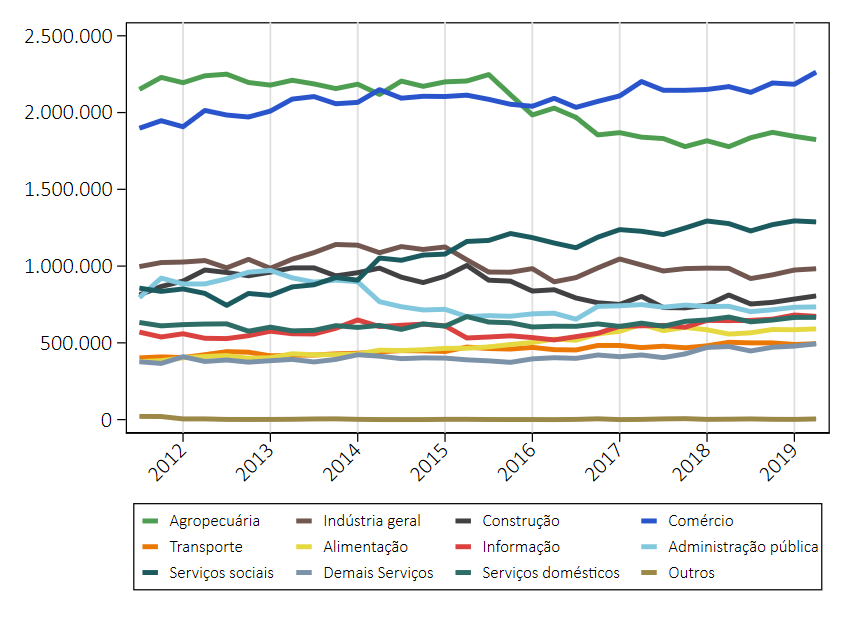
\includegraphics[width=.85\linewidth]{./../analysis/output/_importancia_relativa.png}
  \label{_importancia_relativa}
  \caption{{Número de ocupações por setor econômico}}
\end{figure}
\end{frame}

\section{Amazônia Legal}

\begin{frame}[label=amzcod2dig]{}
\textit{\hyperlink{indice_principal}{\beamerbutton{Voltar}}}
\input{./../analysis/output/amzcod2dig}
\end{frame}

\begin{frame}[label=amzcnae2dig]{}
\textit{\hyperlink{indice_principal}{\beamerbutton{Voltar}}}
\input{./../analysis/output/amzcnae2dig}
\end{frame}

\section{Amapá}

\begin{frame}[label=amzapcod2dig]{}
\textit{\hyperlink{indice_principal}{\beamerbutton{Voltar}}}
\input{./../analysis/output/amzapcod2dig}
\end{frame}

\begin{frame}[label=amzapcnae2dig]{}
\textit{\hyperlink{indice_principal}{\beamerbutton{Voltar}}}
\input{./../analysis/output/amzapcnae2dig}
\end{frame}

\section{Amazonas}

\begin{frame}[label=amzamcod2dig]{}
\textit{\hyperlink{indice_principal}{\beamerbutton{Voltar}}}
\input{./../analysis/output/amzamcod2dig}
\end{frame}

\begin{frame}[label=amzamcnae2dig]{}
\textit{\hyperlink{indice_principal}{\beamerbutton{Voltar}}}
\input{./../analysis/output/amzamcnae2dig}
\end{frame}

\section{Acre}


\begin{frame}[label=amzaccod2dig]{}
\textit{\hyperlink{indice_principal}{\beamerbutton{Voltar}}}
\input{./../analysis/output/amzaccod2dig}
\end{frame}

\begin{frame}[label=amzaccnae2dig]{}
\textit{\hyperlink{indice_principal}{\beamerbutton{Voltar}}}
\input{./../analysis/output/amzaccnae2dig}
\end{frame}

\section{Mato Grosso}

\begin{frame}[label=amzmtcod2dig]{}
\textit{\hyperlink{indice_principal}{\beamerbutton{Voltar}}}
\input{./../analysis/output/amzmtcod2dig}
\end{frame}

\begin{frame}[label=amzmtcnae2dig]{}
\textit{\hyperlink{indice_principal}{\beamerbutton{Voltar}}}
\input{./../analysis/output/amzmtcnae2dig}
\end{frame}

\section{Pará}

\begin{frame}[label=amzpacod2dig]{}
\textit{\hyperlink{indice_principal}{\beamerbutton{Voltar}}}
\input{./../analysis/output/amzpacod2dig}
\end{frame}

\begin{frame}[label=amzpacnae2dig]{}
\textit{\hyperlink{indice_principal}{\beamerbutton{Voltar}}}
\input{./../analysis/output/amzpacnae2dig}
\end{frame}

\section{Rondônia}


\begin{frame}[label=amzrocod2dig]{}
\textit{\hyperlink{indice_principal}{\beamerbutton{Voltar}}}
\input{./../analysis/output/amzrocod2dig}
\end{frame}

\begin{frame}[label=amzrocnae2dig]{}
\textit{\hyperlink{indice_principal}{\beamerbutton{Voltar}}}
\input{./../analysis/output/amzrocnae2dig}
\end{frame}

\section{Rondônia}


\begin{frame}[label=amzrrcod2dig]{}
\textit{\hyperlink{indice_principal}{\beamerbutton{Voltar}}}
\input{./../analysis/output/amzrrcod2dig}
\end{frame}

\begin{frame}[label=amzrrcnae2dig]{}
\textit{\hyperlink{indice_principal}{\beamerbutton{Voltar}}}
\input{./../analysis/output/amzrrcnae2dig}
\end{frame}

\section{Tocantins}


\begin{frame}[label=amztocod2dig]{}
\textit{\hyperlink{indice_principal}{\beamerbutton{Voltar}}}
\input{./../analysis/output/amztocod2dig}
\end{frame}

\begin{frame}[label=amztocnae2dig]{}
\textit{\hyperlink{indice_principal}{\beamerbutton{Voltar}}}
\input{./../analysis/output/amztocnae2dig}
\end{frame}

\section{Manaus}


\begin{frame}[label=amzmanauscod2dig]{}
\textit{\hyperlink{indice_principal}{\beamerbutton{Voltar}}}
\input{./../analysis/output/amzmanauscod2dig}
\end{frame}

\begin{frame}[label=amzmanauscnae2dig]{}
\textit{\hyperlink{indice_principal}{\beamerbutton{Voltar}}}
\input{./../analysis/output/amzmanauscnae2dig}
\end{frame}

\section{Região Metropolitana}


\begin{frame}[label=amzmetropolitanacod2dig]{}
\textit{\hyperlink{indice_principal}{\beamerbutton{Voltar}}}
\input{./../analysis/output/amzmetropolitanacod2dig}
\end{frame}

\begin{frame}[label=amzmetropolitanacnae2dig]{}
\textit{\hyperlink{indice_principal}{\beamerbutton{Voltar}}}
\input{./../analysis/output/amzmetropolitanacnae2dig}
\end{frame}

\section{Zona Rural}


\begin{frame}[label=amzruralcod2dig]{}
\textit{\hyperlink{indice_principal}{\beamerbutton{Voltar}}}
\input{./../analysis/output/amzruralcod2dig}
\end{frame}

\begin{frame}[label=amzruralcnae2dig]{}
\textit{\hyperlink{indice_principal}{\beamerbutton{Voltar}}}
\input{./../analysis/output/amzruralcnae2dig}
\end{frame}

\section{Jovens}


\begin{frame}[label=amzjovemcod2dig]{}
\textit{\hyperlink{indice_principal}{\beamerbutton{Voltar}}}
\input{./../analysis/output/amzjovemcod2dig}
\end{frame}

\begin{frame}[label=amzjovemcnae2dig]{}
\textit{\hyperlink{indice_principal}{\beamerbutton{Voltar}}}
\input{./../analysis/output/amzjovemcnae2dig}
\end{frame}


\section{Comentários}

\frame
{
\begin{center}
	\vfill
	\textbf{Obrigado!}
	\\
	\vfill     
\end{center}
}

\end{document}

